\section{Information Extraction Modules}\label{sec:approach}
In this section, we describe the implementation details of three information extraction modules. Compared with previous approaches~\cite{DBLP:journals/tvcg/HarperA18, DBLP:conf/uist/HarperA14}, our approach has highly significant advantages in adaptability. Specifically, our implementation only requires several accessible inputs by using existing network traffic investigation tools. By using a result-driven approach, our concept regards the creation of node-link diagrams as an invisible ``BlackBox''. It does not depend on any visualization library such as D3~\cite{DBLP:journals/tvcg/BostockOH11} and Vega-Lite~\cite{DBLP:journals/tvcg/SatyanarayanMWH17}, and thus can be utilized to process a diverse variety of visualization programs. Such design enables high adaptability to search different link conditions, summarize complicated visual encoding, and identify different layout results. To maintain consistency, we organize the three modules using the same structure as Section~\ref{sec:overview}.

\subsection {M1: Link Condition Search Module}

Unlike the existing techniques to construct links by selecting link conditions between data entities (nodes), our method infers link conditions based on already constructed links, which reverses the construction process. It extends the application of existing techniques to visualization deconstruction for comprehensibility enhancement.
To be specific, this module consists of three main steps listed below:
% 1) search candidate link conditions in every pair of nodes, 2) filter out the wrong conditions, and 3) store the remaining conditions with a priority, where a more detailed condition gets a higher ranking.

\noindent \textbf{M1.1 Search Candidate Link Conditions}. 
We first constructed conditions between all pairs of nodes. We chose the taxonomy of Graphiti~\cite{DBLP:journals/tvcg/SrinivasanPEB18} to categorize conditions into four types (Summarized in Table~\ref{tab:template}, Link Conditions C1-4). We formalized the conditions with three aspects to facilitate comparison, sorting and filtering.
One condition can be defined as:
\begin{equation}
    \abovedisplayskip=5pt
    \abovedisplayshortskip=5pt
    \belowdisplayskip=5pt
    \belowdisplayshortskip=5pt
    linking\text{ }condition := ( type, attribute, value ) \label{def:linkingcondition}
\end{equation}
where $type$ is the condition type, $attribute$ is the name of the attribute, $value$ is the value of the attribute when the condition holds.
For example, two movies sharing the same actors Alice and Bob are connected under the Condition \textbf{C2}, which could be represented as: ($type$=C2, $attribute$=actors, $value$=[Alice, Bob]). 

\noindent \textbf{M1.2 Filter Out Wrong Conditions}.
After searching candidate link conditions, current conditions are established on all node pairs despite no connection between two nodes.
Considering our goal is to detect conditions which only exist on node pairs, which are connected by links, we need to remove conditions held on node pairs without links. After that, only conditions with the least number of links will be selected from the remaining conditions.

\noindent \textbf{M1.3 Sort Remaining Conditions}.
After that, conditions are sorted with a priority, 
where the more detailed the condition, the higher its ranking.
For example, the condition ($type$=C2, $attribute$=actors, $value$=[Alice, Bob]) is implied by ($type$=C2, $attribute$=actors, $value$=arbitrary), where ($value$=arbitrary) means the condition does not assume the $actors$ should be of a certain value.
The former condition is more specific than the latter, and is thus ranked higher.
The highest-ranked condition is regarded as the most likely condition.

\begin{algorithm}[tp]
    \renewcommand\arraystretch{1.2}
    \caption{ Link Condition Search }
    \setlength{\belowcaptionskip}{-15pt}
    \label{alg:conditions}
    \begin{algorithmic}[1]
        \Require
            $G=(V=\{v_1, v_2, ..., v_n\}, E=\{e_1, e_2, ..., e_n\})$: a graph
        \Ensure
            $C$: the potential condition set
        \State Init conditions $C=\varnothing$, false conditions $FC=\varnothing$
        \For {each node pair $(v_i, v_j)$}
            \State $C_{ij} \gets$ all conditions that can connect $(v_i, v_j)$
            \If {$(v_i, v_j)$ is not a link}
                \State merge $FC$ with $C_{ij}$
            \Else
                \State merge $C$ with $C_{ij}$
            \EndIf
        \EndFor
        \State remove $FC$ from $C$
        \For {each condition $c$ in the condition set $C$}
            \If {the frequency of $c$ is less than $|E|$}
                \State remove $c$ from $C$
            \EndIf
        \EndFor
        \State sort $C$
        \State \Return $C$
    \end{algorithmic}
\end{algorithm}

\subsection{\textbf{M2: }Visual Encodings Summarization Module}\label{sec:visualencodings}
Our module summarizes visual encodings from node-link diagrams in the SVG format, which is widely used in the visualization area~\cite{DBLP:journals/tvcg/BostockOH11, sievert2017plotly, DBLP:journals/vi/WangBLDFPC21}.
To enlarge the usage scenario of this module, we did not make the algorithm rely on any library.

Attributes of nodes and links are usually encoded by visual channels to reveal attribute-based patterns.
Nodes and links contained in the underlying graph are denoted as \textit{data entities}, and each data entity consists of several \textit{attributes}.
For example, in the node-link diagram example (Figure~\ref{fig:VisualEncodings}), a node contains a categorical attribute (\textit{x}) and a numerical list attribute (\textit{y}). We encode the attribute \textit{y} with the height of two rectangles.
Then we encode the attribute \textit{x} with the two rectangles' fill color and the background rectangle's stroke color.
Visualization creators can write programs with the W3C DOM API to construct visualizations within SVG.
A SVG includes a root element \texttt{<svg>} and allows hierarchical grouping of sub-elements with group elements \texttt{<g>}.
Marks onscreen are generated by graphical elements, such as \texttt{<rect>}, \texttt{<circle>}, and \texttt{<ellipse>}.
We call these graphical elements \textit{visual elements}.
Their style attributes such as cx, cy, width, and height are denoted as \textit{visual channels}. We formulate the encoding scheme as:
\begin{equation}
    \abovedisplayskip=5pt
    \abovedisplayshortskip=5pt
    \belowdisplayskip=5pt
    \belowdisplayshortskip=5pt
    encoding := (entity, attribute, element, channel) \label{def:encoding}
\end{equation}


\begin{figure}[tp]
    \centering
    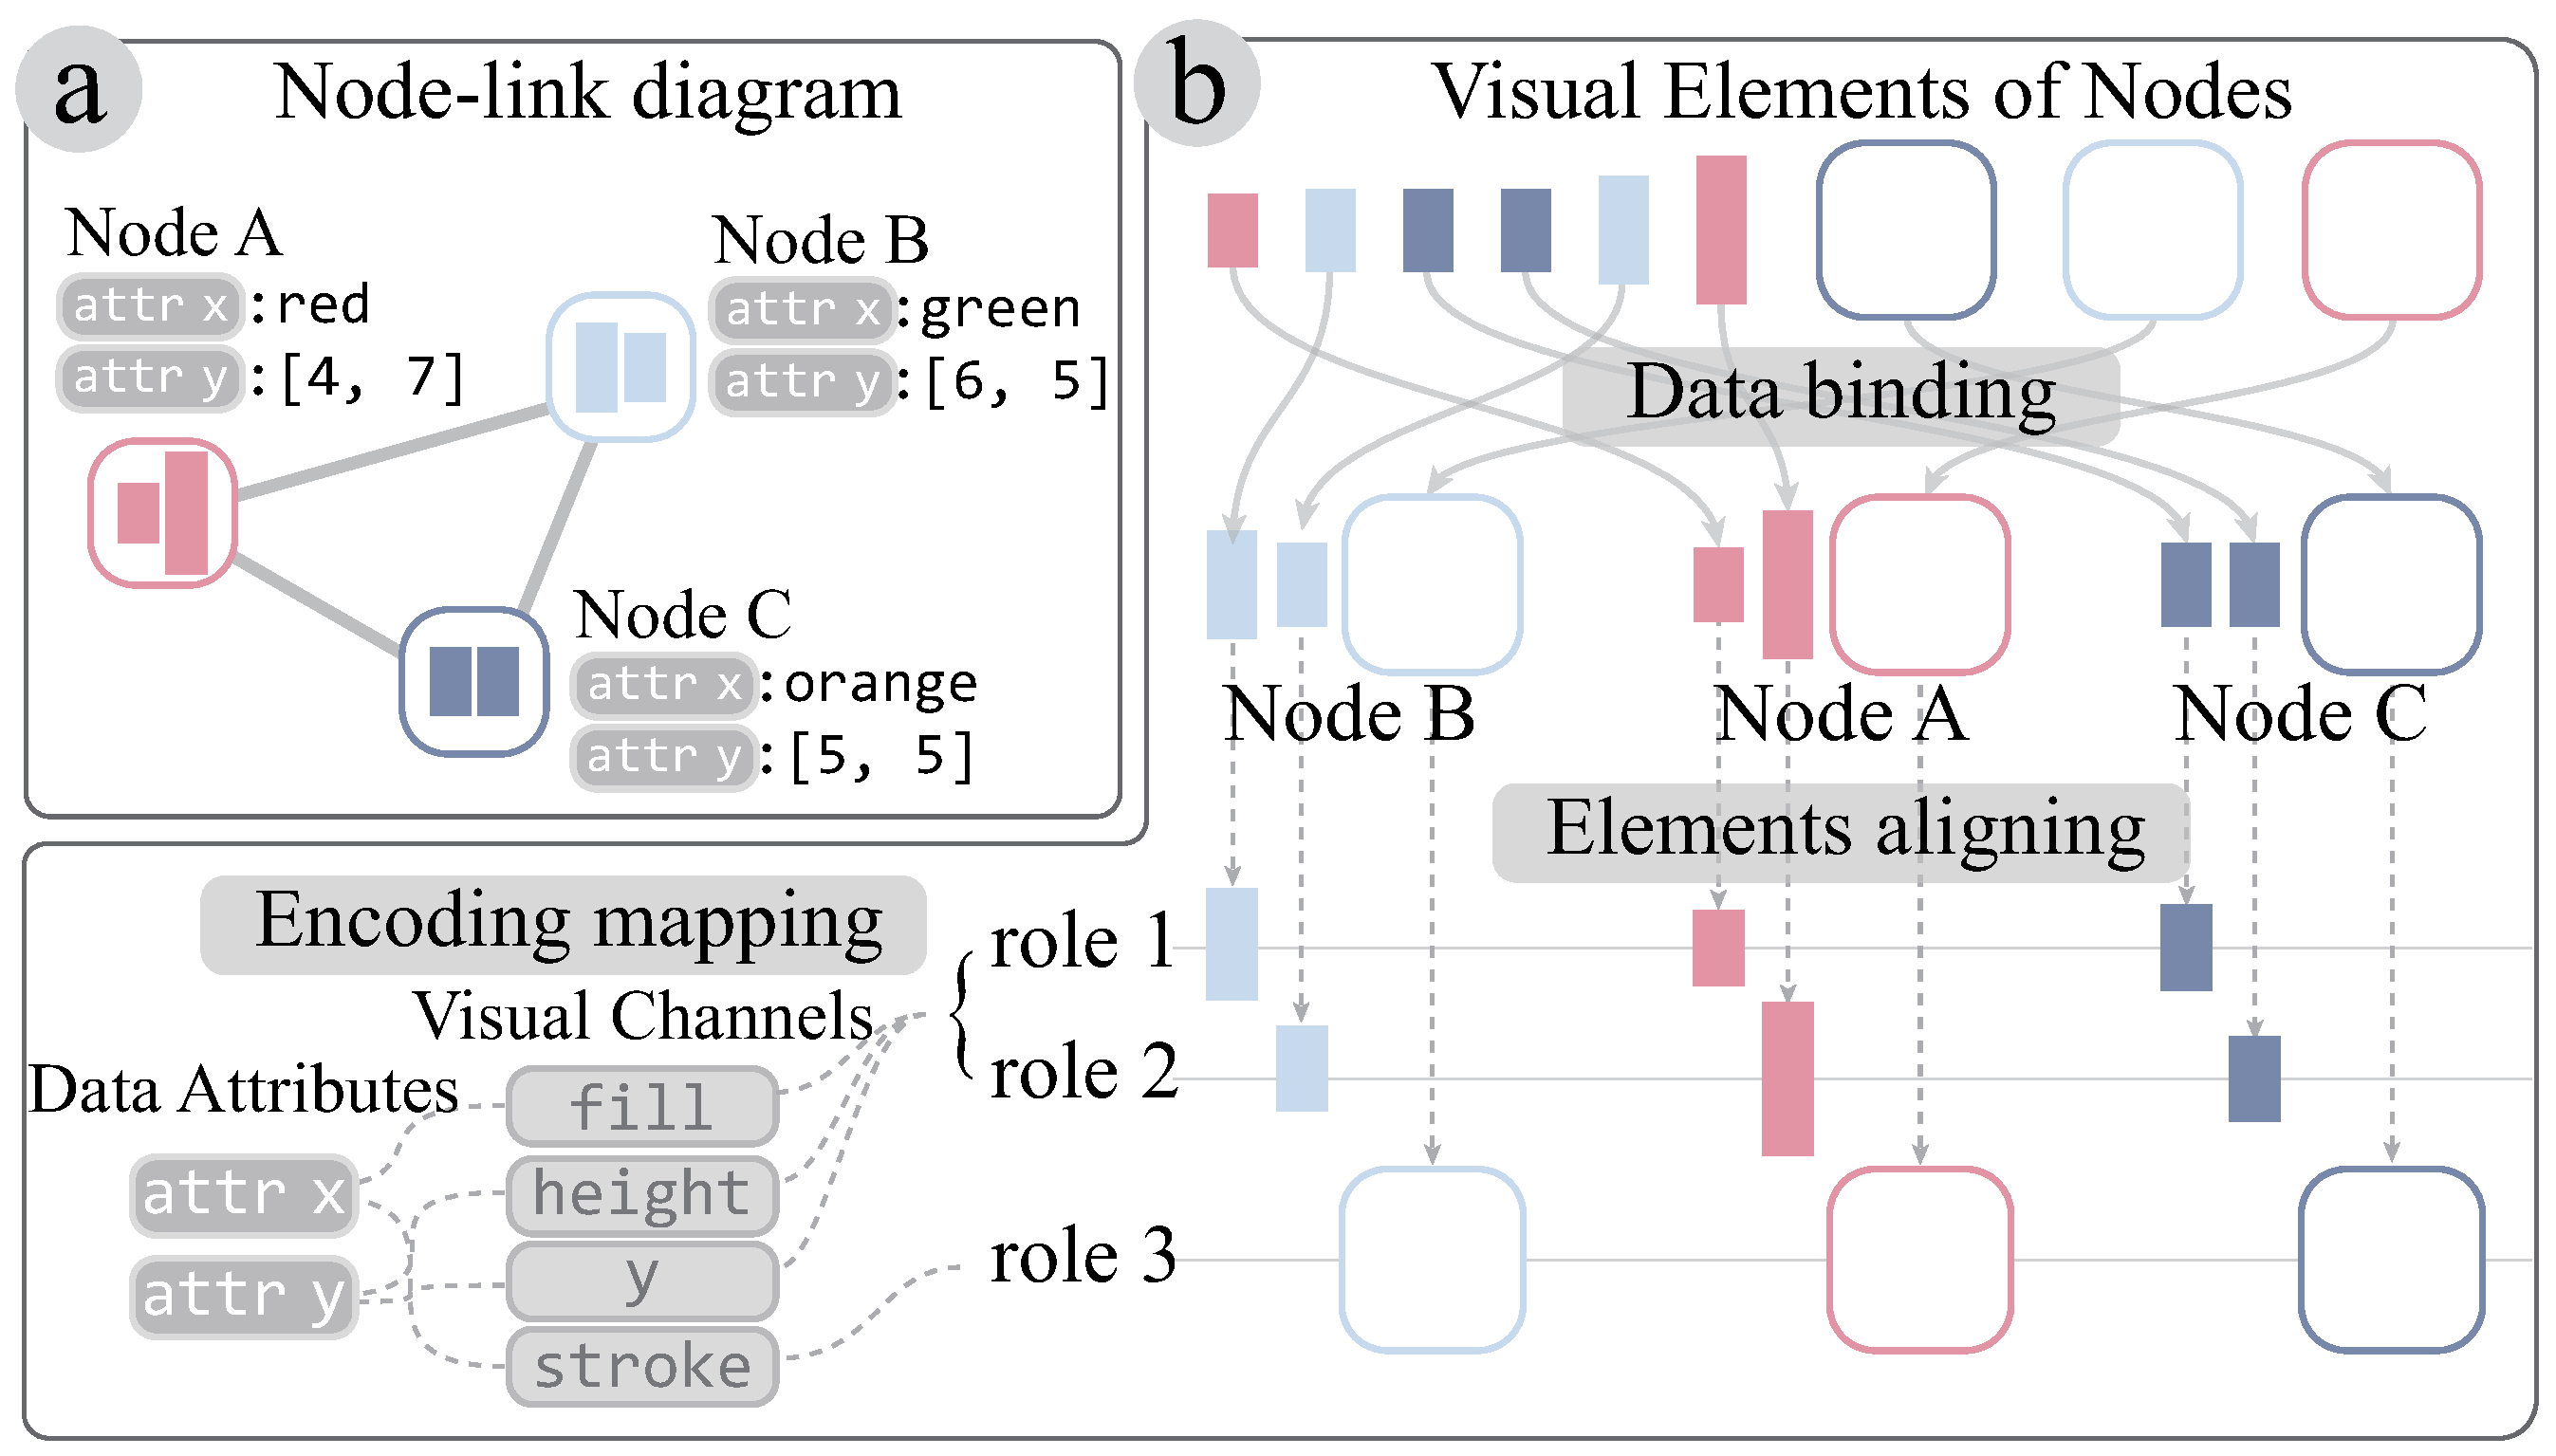
\includegraphics[width=1\columnwidth]{figures/VisualEncodings.eps}
    \setlength{\belowcaptionskip}{-10pt}
    \caption{How \ApproachName~summarizes visual encodings from a node-link diagram in the SVG format. (a) A node-link diagram consists of three nodes and three links (upper left corner). (b) Node elements are extracted and the data binding step (mapping visual elements to node entities)
    % maps them into different node entities. Then elements having the same role across different node entities are aligned into the same role class in the 2.
    the elements aligning step (aligning visual elements according to their roles),
    % Mappings among roles, visual channels, and attributes are detected by the 3.
    and the encoding mapping step (mapping data attributes to visual channels).}
    \label{fig:VisualEncodings}
\end{figure}

\begin{figure}[tp]
    \centering
    \setlength{\belowcaptionskip}{-10pt}
    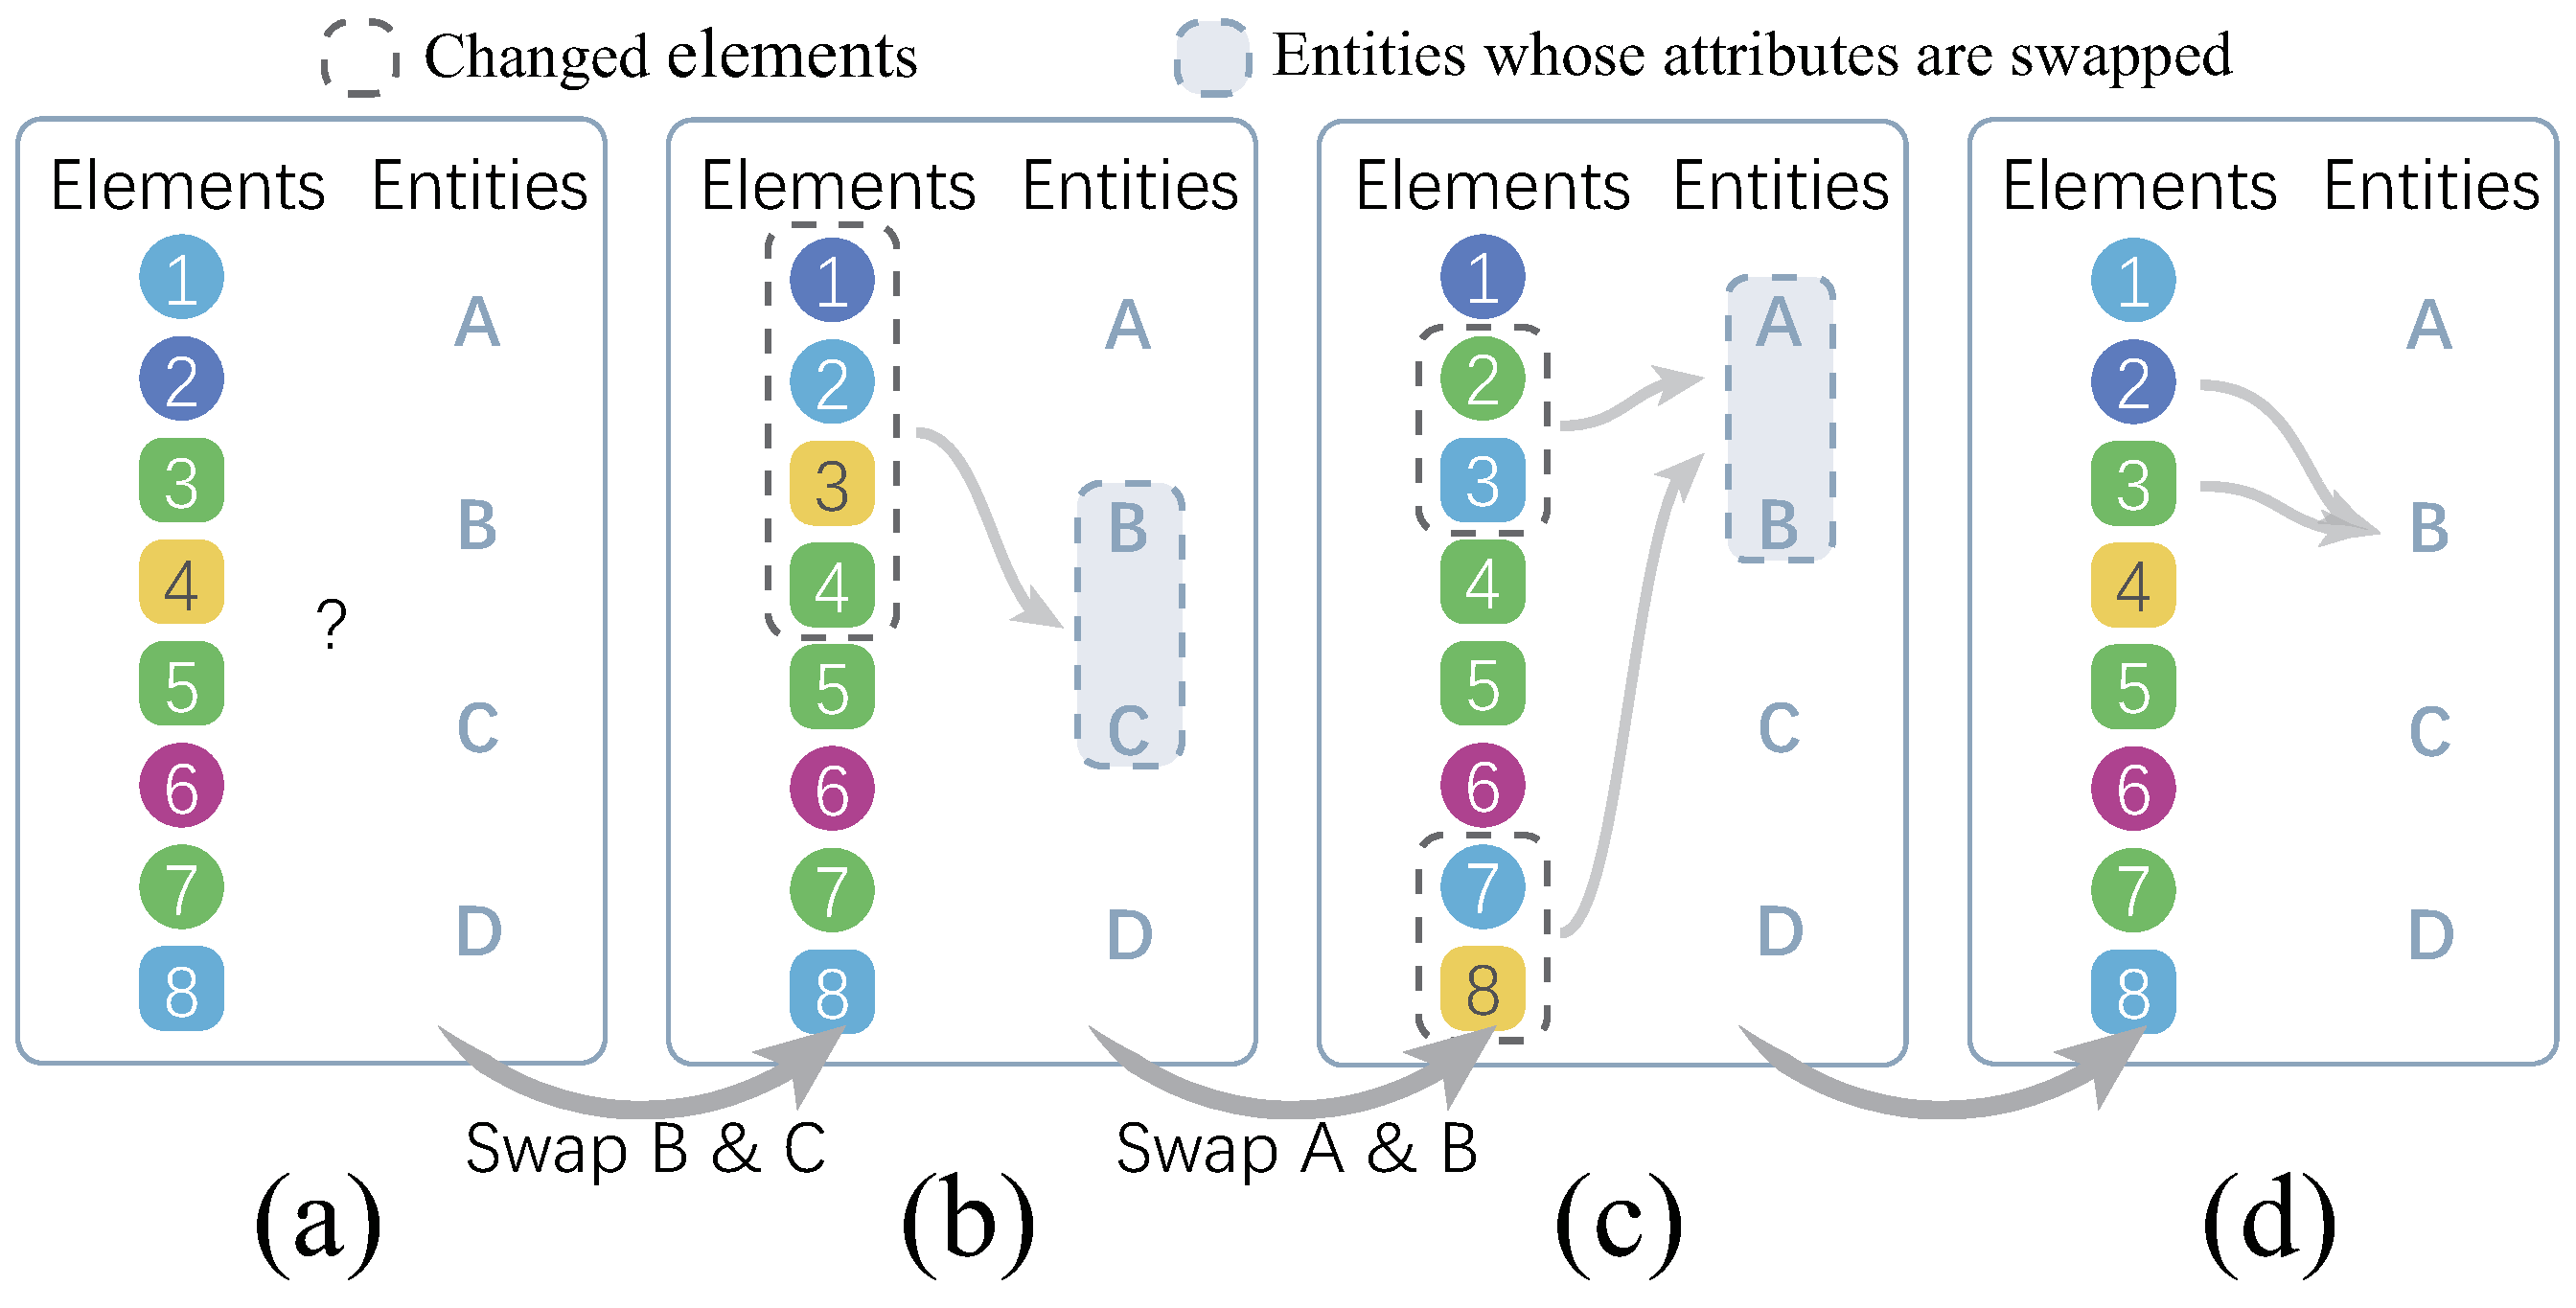
\includegraphics[width=1\columnwidth]{figures/DataBinding.eps}
    \caption{ The Data binding is achieved by swapping entities. 
    % At first, visual mappings between original visual elements and data entities are unknown. Swapping attributes of entities B and C influences the appearance of elements 1 to 4. Thus, B and C correspond to 1 to 4. Them, swapping attributes of  A and B influences 2, 3, 7, and 8. Thus, A and B correspond to these elements. Swapping B with A and C changes elements 2 and 3 twice. Thus, we map entity B to elements 2 and 3.
    }
    \label{fig:DataBinding}
    % \setlength{\abovecaptionskip}{-100pt}
    % \setlength{\belowcaptionskip}{-100pt}
\end{figure}

\begin{figure}[tp]
    \centering
    \setlength{\belowcaptionskip}{-10pt}
    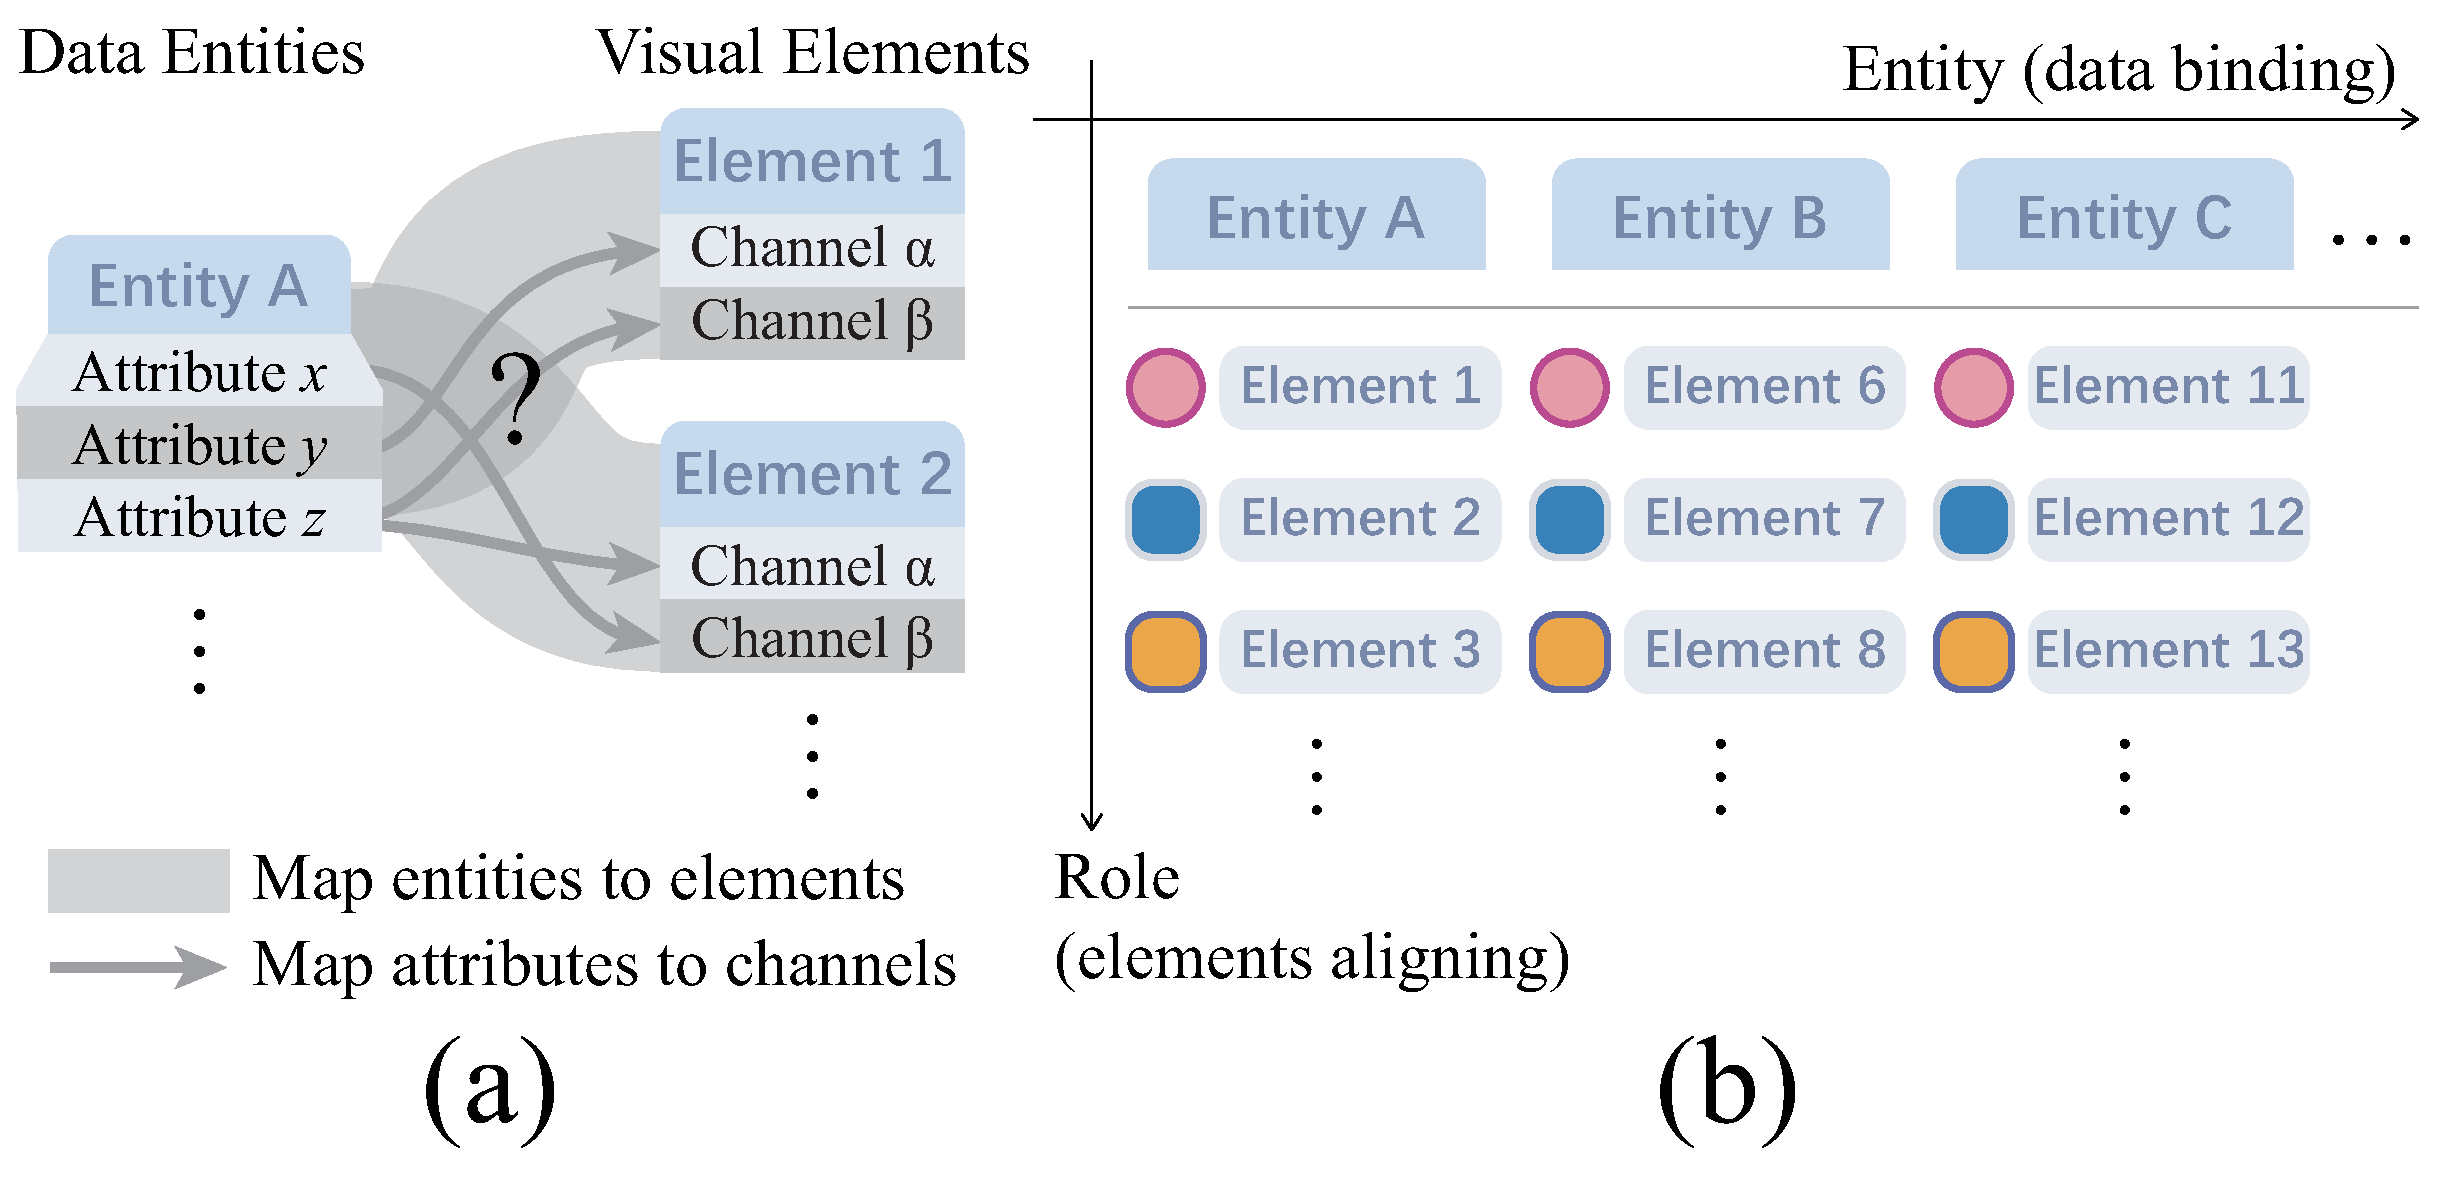
\includegraphics[width=1\columnwidth]{figures/ElementAligning.eps}
    \caption{The target of our visual encoding summarization module.
    (a) The target of the module is to find mappings among data entities, visual elements, data attributes, and visual channels. (b) To achieve the target, we utilize the data-binding step and the elements-aligning step to clarify the entity and the role of each visual element.}
    \label{fig:ElementAligning}
\end{figure}




{\bf M2.1 Data Binding.} \label{sec:databinding}
To detect mappings between \textit{data entities} and \textit{visual elements}, we modified attribute values of data entities and recorded corresponding visual element changes to construct mappings between them.
% For example, the node's \texttt{size} attribute is linearly mapped into the radius of the \texttt{<circle>} element encoding the node: 
% $radius_i = (size_i - min(size)) / (max(size) - min(size)) * radius_{max}$.
% Directly modifying $size_i$ may broaden the attribute range and changes the linear mapping defined by the attribute range.
% So that elements related to other data entities may also be changed.
% We prevent this by merely swapping attributes of the two entities rather than modifying them, so that no new data is introduced, and the distribution is preserved.
To prevent changing the distribution of attribute values, we merely swap attributes of the two entities rather than modifying them.
After swapping all two entities' attributes, visual elements that differ from the previous are regarded as two entities' corresponding elements.
For example, in Figure~\ref{fig:DataBinding} after swapping nodes B and C, elements 1 to 4 are changed.
All these changed elements correspond to nodes B and C because only B and C are modified. Then, after swapping the node B with A, elements 2 and 3 are changed twice. Thus they correspond to node B because only node B was swapped twice. Each node will be swapped with all other nodes to ensure detecting all elements belonging to it. After swapping all nodes, the entire node-to-element mapping is constructed. Thus, node entities are bound to their corresponding elements. The link-to-element mapping is constructed in the same way. Because swapping two nodes may influence their related links, node elements currently contains elements of their related links. We remove link elements from the node-to-element mappings. Two parts (\textit{entity} and \textit{element}) of the mapping relationship are solved.


{\bf M2.2 Elements Aligning.}
The data-binding step only binds visual elements into different data entities (the horizontal direction in Figure~\ref{fig:ElementAligning}b).
The roles of different elements are unknown.
The \textit{role} of an element is identified by its function in the visualization process.
We define the \textit{role} as a function that maps attributes to visual channels:
\begin{equation}
    \abovedisplayskip=5pt
    \abovedisplayshortskip=5pt
    \belowdisplayskip=5pt
    \belowdisplayshortskip=5pt
    role :=  \{attribute: value\} \mapsto \{channel: appearance\}
\end{equation}
Two elements have the same role if, given arbitrary, same inputs (all attributes of their corresponding entities) produce same outputs (all their visual channels).
For the example in Figure~\ref{fig:VisualEncodings}, 
the roles of all three left bars in node A, B, and C are the same,
because they encode same attributes with same visual channels.
% we swap all attributes of nodes A and B, node A's left rectangle before swapping will be the same as node B's left rectangle after swapping regarding all their visual channels such as x, y, fill, and height.
They are aligned to classify their roles (the vertical direction in Figure~\ref{fig:ElementAligning}b).
We determine the role of each element by swapping its data entity with others. Two elements of the same role behave the same after exchanging their data entities.
% Different elements' role identity can be determined by swapping their corresponding data entities along with the data binding step, because all attributes of one entity before swapping are the same to the counterpart of the other one after swapping.
% For instance, in Figure~\ref{fig:DataBinding}b, after swapping entity B with entity C, element 1 appears the same as element 2 before swapping in Figure~\ref{fig:DataBinding}a. Thus, elements 1 and 2 can be aligned into the same role.
We clarify the binding among visual elements, data attributes, and visual channels, which is conducive to the subsequent steps.


{\bf M2.3 Encoding mapping.}\label{sec:encodingmapping}
The previous two steps align elements according to two dimensions (the entity and the role) to clarify the relationship between data entities and visual elements.
However, correlations between visual channels and data attributes are not determined.
We detected related visual channels of an attribute by shuffling it of  all data entities and observing changes of their corresponding elements.
One correlation is defined as ``which \textit{attribute} changes which \textit{visual channel} of which \textit{element}''. We formalize it as:
\begin{equation}
    \abovedisplayskip=5pt
    \abovedisplayshortskip=5pt
    \belowdisplayskip=5pt
    \belowdisplayshortskip=5pt
    correlation := ( attribute, element, channel )
\end{equation}
We merge different correlations according to the role of elements.
Moreover, we identify the category of correlations to clarify correlations between visual channels and data attributes.
It requires the classification of attribute types and channel types.
We support numerical attributes and categorical attributes.
List attributes and dictionary attributes are separated into multiple numerical attributes or categorical attributes (e.g.,[1, 2, 3], \{"year":2021,"month":03\}).
We regard all visual channels as numerical (colors can be divided into RGB channels, which are numerical).
However, numerical data can be used as categorical data if there are only a few unique values (less than $\alpha\%$).
% For example, natural numbers are often used as categorical attributes such as labels, groups, and classes.
% Thus, for numerical data, we must compare the number of unique values and their entries to determine whether it is numerical or categorical.
% We set up a parameter $\alpha$ to make the distinction: if all values of the attribute are natural numbers and
% the number of an attribute's unique values is less than $\alpha$ a percent of the number of data entities, we regard the attribute as categorical.
We identify the type of correlation by attribute and channel types:

\noindent \textbf{Categorical correlation} -- the channel and attribute are both categorical or the channel is categorical while the attribute is numerical. 
To summarize the correlation of different channel values, we record the value range of the attribute for each channel values.
    
\noindent \textbf{Numerical correlation} -- the channel and attribute are both numerical. We compute the Pearson's Correlation Coefficient and test whether the correlation is positive, negative, or uncorrelated with the coefficient and the significance test's p-value.  The correlation is built when the absolute value of the coefficient is larger than $\theta$=.5, and the $p$-value is less than $\alpha$=.05. Both parameters can be adjusted on-demand.

We do not support the correlation type where the channel is numerical while the attribute is categorical because the former is continuous and the latter is discrete. It is counterintuitive.

\subsection{\textbf{M3}: Layout Type Identification Module}


\textbf{M3.1 Capturing the position of each node}.
Node positions are used to determine the layout type.
To capture each node's position, we compute a bounding box for elements detected in the \textbf{Data Binding} step.
It is the smallest rectangle that contains all corresponding elements.
We take its centroid as the position of the node.

\textbf{M3.2 Determining the layout type.} 
Topology-driven layouts prioritize the topology of a graph~\cite{DBLP:journals/cgf/NobreMSL19}, which means their graph geodesic distance influences the Euclidean distance between two nodes. To validate this assumption, we performed a study by using the Pearson test to check the correlation between the geodesic distance and the Euclidean distance in 15 graphs from~\cite{DBLP:journals/tvcg/ZhuCHHLZ21} layered by five topology-based layouts with default parameters (FM$^3$~\cite{hachul2004drawing}, Fruchterman-Reingold spring layout (F.R.)~\cite{DBLP:journals/spe/FruchtermanR91}, Stress Majorization (S.M.)~\cite{DBLP:conf/gd/GansnerKN04}, Pivot MDS (PMDS)~\cite{DBLP:conf/gd/BrandesP06}, and Radial Tree layout (R.T.)~\cite{DBLP:conf/infovis/Jankun-KellyM03}).
Over the total $15 \times 5 = 75$ trials, only coefficients of seven trials were less than $\theta = .5$ (see Supplementary Materials 1). And $p$-values were all zero for the five topology-based layouts in all 15 datasets.
The result indicates that in most cases, the Euclidean distance between two nodes reflects their graph geodesic distance with topology-based layouts.
Thus, it is feasible to study whether the layout is a topological layout using the Pearson correlation test.

The attribute-driven layout category consists of algorithms that map node attributes to the two dimensions ($x$ and $y$) of the Cartesian coordinate. 
We applied the Pearson correlation test to Section~\ref{sec:encodingmapping} similarly to test whether an attribute relates to the layout.

To determine the layout type, we utilize the Pearson correlation coefficient. If coefficients of the two layout types are both less than a threshold $\theta < .5$, we suggested there is no certain layout in the node-link diagram. Otherwise, the layout type with a larger coefficient is regarded as the actual layout. 